\section{Non-parametric Bayesian Inference (BI)}

\subsection*{Exact Conjugate Prior of Multivariate Gaussian}
Data: $x_i\sim \mathcal{N}(\mu,\Sigma)$ i.i.d.. Inverse Wishart: $\Sigma \sim \mathcal{W}^{-1}(S, v) \propto |\Sigma|^{(v+p+1)/2}$ $\exp( - \operatorname{Tr}( \Sigma^{-1} S)/2 )$. \\
\textbf{Normal Inverse Wishart} as conjugate prior: $p(\mu, \Sigma | m_0, k_0, v_0, S_0) = \mathcal{N}(\mu | m, \Sigma/k_0)\mathcal{W}^{-1}(\Sigma | S_0,v_0)$. 

Update rule: \begin{footnotesize}
    $m_p = (k_0 m_0+N\bar{x})/(k_0+N)$, $k_p = k_0 + N$, $v_p =v_0 + N$, $S_p =S_0 + k_0 m_0 m_0^{\top} - k_p m_p m_p^{\top} + \sum (x_i-\bar{x})(x_i-\bar{x})^{\top}$. 
\end{footnotesize}


\subsection*{BI with Semi-Conjugate Prior}
New prior: $\mu$\textasciitilde$ \mathcal{N}(m_0,V_0)$, $\Sigma $\textasciitilde$ \mathcal{W}^{-1}(S_0, v_0)$, then posterior $p(\mu,\Sigma | X)$ is intractable, but condition posterior is exact, \begin{footnotesize}
    $p(\mu | \Sigma, X) = \mathcal{N}(m_p,V_p)$, $V_p^{-1} = V_0^{-1} + N\Sigma^{-1}$, $V_p^{-1}m_p = V_0^{-1} m_0 + N\Sigma^{-1}\bar{x}$; $p(\Sigma | \mu, X) = \mathcal{W}^{-1}(S_p,v_p)$, $v_p = v_0 + N$, $S_p = S_0 +\sum x_ix_i^{\top} + N\mu\mu^{\top} - 2N\bar{x}\mu^{\top}$. 
\end{footnotesize}

\textbf{Gibbs sampling}: random variable $p(z_1,\cdots, z_p)$ intractable, cyclically resample $z_i$ according to tractable conditional distribution $p(z_i | z_{/i})$ $n$ times, when $n\to \infty$, $(z_1,\cdots, z_p)$\textasciitilde$ p(z_1,\cdots, z_p)$ 

Finally, replace posterior with MC sampling: $\mathbb{E}_{\theta | X} f(x| \theta) \approx \sum f(x| \theta_i) / N$

\subsection*{BI for Gaussian Mixture Model}
Data model: latent $K$ class variable $z_i $\textasciitilde$ \operatorname{Cat}(\pi)$, observed $x_i$\textasciitilde$ \mathcal{N}(\mu_{z_i}, \Sigma_{z_i})$. Prior: $\mu_k $\textasciitilde$ \mathcal{N}(m_0,V_0)$, $\Sigma_k $\textasciitilde$ \mathcal{W}^{-1}(S_0, v_0)$, $\pi$\textasciitilde$ \operatorname{Dir}(\alpha)\propto\prod_k^{K} p_{k}^{\alpha_k-1}$. Prior also intractable. 

\textbf{Goal} Gibbs sampling for BI, but to simplify conditional distribution.
\vspace{-0.3cm}
\begin{center}
    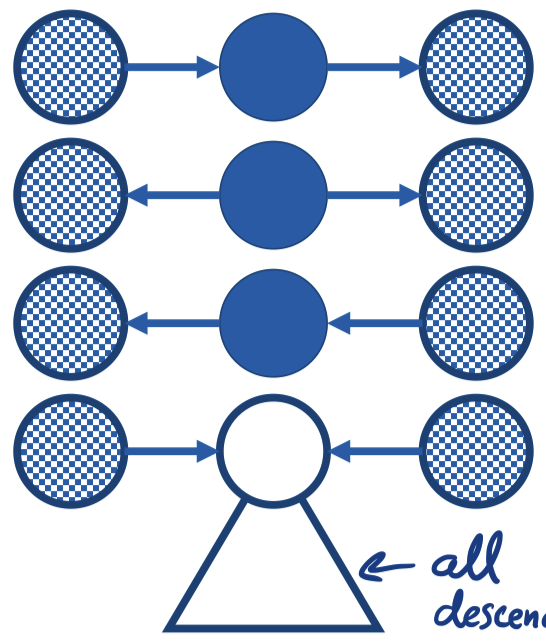
\includegraphics[width=0.25\columnwidth]{figures/d-sep.png}
    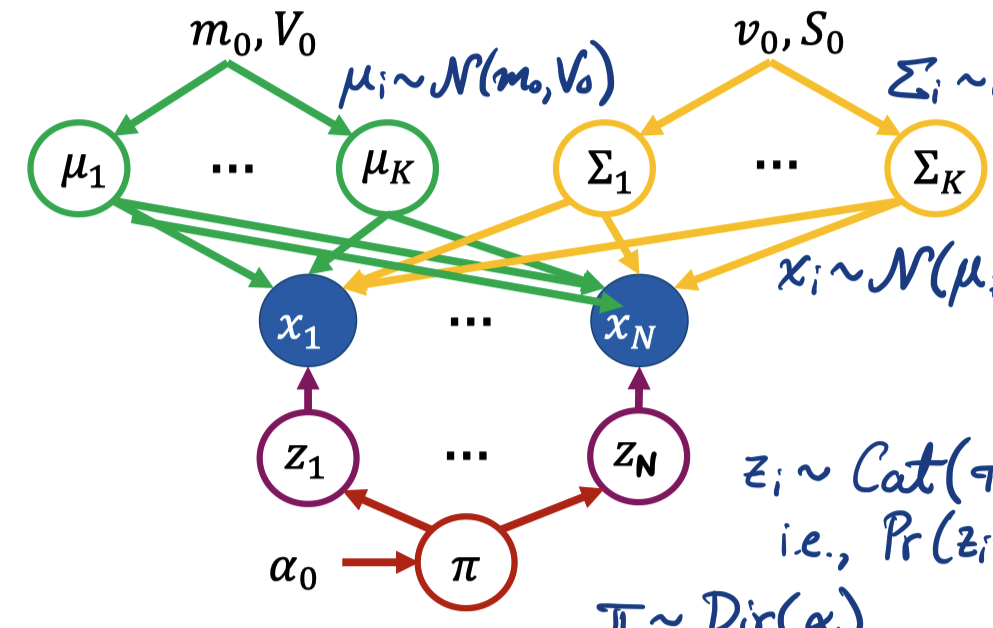
\includegraphics[width=0.4\columnwidth]{figures/GMM.png}
\end{center}
\vspace{-0.4cm}

\textbf{d-seperation}: for verifying conditional independence. Given with observed variable set $C$, if every path from variable $A$ to $B$ is blocked on probability graph, then $A$ and $B$ are independent condition on $C$. By this thm: (1) $z_i$, $z_j$ (2) $\mu$, $\pi$  (3) $\Sigma$, $\pi$ all independent condition on other parameter. Sampling procedure: 
    (1) $z^{(t)} \leftarrow p\left(\cdot | x, \mu^{(t-1)}, \Sigma^{(t-1)}\right)$, (2) $\mu^{(t)} \leftarrow p\left(\cdot | x, \Sigma^{(t-1)}, z^{(t)}\right)$, (3) $\Sigma^{(t)} \leftarrow p\left(\cdot | x, \mu^{(t)}, z^{(t)}\right)$, (4) $\pi^{(t)} \leftarrow p\left(\cdot | x, z^{(t)}\right)$

\subsection*{BI for Non-Parametric GMM}
\textbf{Goal}: sample from infinite categorical distri.

\textbf{Dirichlet Process (DP)}: $\Theta$ parameter space, $H$ prior distri on $\Theta$, $A_1, \cdots, A_r$ arbitrary partition of $\Theta$. $G$ a categorical distribution over $\{A_i\}$ is  $G $\textasciitilde$ \mathrm{DP}(\alpha, H)$ if $\left(G\left(A_{1}\right), \ldots, G\left(A_{r}\right)\right) $\textasciitilde$ \operatorname{Dir}\left(\alpha H\left(A_{1}\right), \ldots, \alpha H\left(A_{r}\right)\right)$.

\textbf{Posterior}: $G | \{\theta_{i}\}_{i=1}^n $\textasciitilde$ \operatorname{DP}\left(\alpha+n, \frac{\alpha H + \sum_{i=1}^{n} \delta_{\theta_{i}}}{\alpha+n}\right)$

\textbf{Condition on $\theta$, Margin over $G$}: $\theta_{n+1} \mid \theta_{1}, \ldots, \theta_{n} $\textasciitilde$ \frac{1}{\alpha+n}\left(\alpha H+\sum_{i=1}^{n} \delta_{\theta_{i}}\right)$, Leads to CRP

\subsection*{Three Methods of Sampling from DP}

In $K\to\infty$ GMM, $\theta$ in DP is $z$, $G$ is $\pi$. 

\textbf{(1) Chinese Restaurant Process (CRP)}, sample $z$, marginalize over $\pi$: \\
$p(z_n = k| \theta_{i < n}) = 
\begin{cases}
    n_k / (\alpha + n - 1) \text{, existing }k \\
    \alpha / (\alpha + n - 1) \text{, new }k 
\end{cases}
$

\textbf{Expect \# of Class} $\sum_{i=1}^{n} \frac{\alpha}{\alpha+i-1} $\textasciitilde$eq \alpha \log \left(1+\frac{n}{\alpha}\right)$

\textbf{(2) Stick-breaking Construction} samples $\pi$: $\beta_{k} $\textasciitilde$ \operatorname{Beta}(1, \alpha)$, $\theta_{k}^{*} $\textasciitilde$ H$, $\pi_{k}=\beta_{k} \prod_{l=1}^{k-1}\left(1-\beta_{l}\right)$

\textbf{(3)} Marginalize over $\mu, \Sigma$ when sampling $z$ (if intractable), less variance (Rao-Blackwall).

\textbf{Exchangeability}: $p(\{\theta_i\}) = \prod_{n=1}^N p(\theta_n | \{\theta_{i<n}\})$ unchanged after permuting sampling order.

\textbf{DeFinetti’s Thm} any exchangeable distri is a mixture model $P\left(\{\theta_{i}\}\right)=\int \prod_{i=1}^{n} G\left(\theta_{i}\right) d P(G)$
